% !TEX root = ../ejemplo-memoria.tex
% Contenidos del capítulo.
% Las secciones presentadas son orientativas y no representan
% necesariamente la organización que debe tener este capítulo.

% filepath: c:\Users\isiva\Documents\memoria_TFG\donammon\tex\estado_arte.tex


\section{Historia, evolución e impacto de las aplicaciones móviles}

\subsection{Origen y evolución de los dispositivos móviles}

El desarrollo de las aplicaciones móviles no puede sin revisar primero la evolución histórica de los dispositivos que las alojan. La telefonía móvil nace en 1946 con el sistema móvil de AT\&T, que permitía realizar llamadas desde vehículos utilizando dispositivos de más de 30 kg. Este sistema inicial, basado en la tecnología Push-To-Talk y gestionado por operadoras humanas, tenía una cobertura muy limitada y altos costes de uso~\cite{agar2004}.

Durante las décadas siguientes se sucedieron avances importantes: la introducción del sistema RCC en 1960, el Improved Mobile Telephone Service de AT\&T en 1965, y finalmente, la llegada del primer teléfono móvil portátil, el Motorola DynaTAC, en 1983. Sin embargo, no fue hasta la década de 1990 cuando los dispositivos comenzaron a incorporar funcionalidades propias de asistentes personales, como los Apple Newton o los Palm Pilot, marcando así el inicio de las primeras ``aplicaciones'' de uso cotidiano, como agendas, calendarios y juegos como Snake de Nokia~\cite{west2010}.

El cambio de paradigma llegó en 2007 con la aparición del iPhone, que introdujo una interfaz multitáctil intuitiva y eliminó el teclado físico, inaugurando así la era del smartphone moderno. Un año más tarde, Apple lanzó la App Store, permitiendo a desarrolladores externos distribuir aplicaciones fácilmente. Ese mismo año, Google presentó Android junto con el HTC Dream, diversificando el ecosistema y facilitando el acceso masivo al desarrollo y consumo de aplicaciones móviles~\cite{murphy2014}.

\subsection{Ecosistemas y sistemas operativos móviles}

El auge de las aplicaciones móviles está estrechamente vinculado al desarrollo de los sistemas operativos (SO) móviles. Durante los primeros años del siglo XXI, Symbian OS dominaba el mercado, especialmente en terminales de Nokia. Sin embargo, fue rápidamente desplazado por iOS (2007) y Android (2008), que ofrecían interfaces gráficas avanzadas, tiendas de aplicaciones centralizadas y acceso optimizado a hardware~\cite{statcounter2024}.

Actualmente, Android posee una cuota de mercado superior al 70\% a nivel global, mientras que iOS concentra cerca del 28\% del mercado, especialmente en países desarrollados~\cite{statista2024}. Otros sistemas operativos como Windows Phone, BlackBerry OS o Tizen han desaparecido o mantienen una presencia marginal. La consolidación de este duopolio ha propiciado estándares de desarrollo bien definidos, facilitando la expansión del mercado de aplicaciones.

Cabe destacar que la fragmentación del ecosistema Android sigue representando un reto técnico. Según un estudio de Android Police~\cite{androidpolice2017}, el tiempo medio de soporte de actualizaciones es de 21 meses en dispositivos Android, frente a los 41 meses de Apple, lo que obliga a los desarrolladores a implementar múltiples versiones y adaptaciones para garantizar la compatibilidad.

\subsection{Tipos de aplicaciones móviles}

Las aplicaciones móviles pueden clasificarse en función de su arquitectura en cinco categorías principales:

\begin{itemize}
    \item \textbf{Aplicaciones web}: ejecutadas dentro del navegador, sin necesidad de instalación. Utilizan tecnologías como HTML5, CSS y JavaScript. Son portables pero con acceso limitado al hardware~\cite{nguyen2018}.
    \item \textbf{Aplicaciones web progresivas (PWA)}: ofrecen una experiencia cercana a las nativas, pueden instalarse desde el navegador y ejecutarse sin conexión, gracias a tecnologías como los service workers.
    \item \textbf{Aplicaciones híbridas}: encapsulan una web app dentro de una aplicación nativa mediante motores como Cordova o Ionic. Permiten cierto acceso a funciones del dispositivo, pero con rendimiento inferior a las apps nativas.
    \item \textbf{Aplicaciones nativas}: desarrolladas específicamente para cada plataforma, usando lenguajes como Swift (iOS), Kotlin o Java (Android). Ofrecen el mejor rendimiento, pero requieren múltiples desarrollos independientes.
    \item \textbf{Aplicaciones nativas multiplataforma}: permiten usar un único lenguaje y base de código para generar versiones para iOS y Android. Ejemplos incluyen React Native, Flutter y Xamarin, ampliamente utilizados en el desarrollo moderno~\cite{gartner2022}.
\end{itemize}

% Definición de colores para la tabla (debe ir antes de la tabla)
\definecolor{verde}{RGB}{0,153,0}
\definecolor{rojo}{RGB}{204,0,0}
\definecolor{marron}{RGB}{153,102,51}

% Tabla comparativa de tipos de aplicaciones móviles
\begin{table}[htbp]
\centering
\renewcommand{\arraystretch}{1.5}
\rowcolors{2}{gray!10}{white}
\begin{tabularx}{\textwidth}{|X|c|c|c|c|}
\hline
\textbf{} & \textbf{App Nativa} & \textbf{App Híbrida} & \textbf{App Web (Progresiva)} & \textbf{App Web} \\
\hline
Experiencia de usuario & \textcolor{verde}{EXCELENTE} & \textcolor{verde}{EXCELENTE} & \textcolor{marron}{BUENA} & \textcolor{rojo}{NORMAL} \\
\hline
Velocidad y Rendimiento & \textcolor{verde}{MUY RÁPIDA} & \textcolor{verde}{MUY RÁPIDA} & \textcolor{marron}{BUENA} & \textcolor{rojo}{NORMAL} \\
\hline
Seguridad & \textcolor{verde}{ALTA} & \textcolor{verde}{ALTA} & \textcolor{marron}{BUENA} & \textcolor{marron}{BUENA} \\
\hline
App Stores & \textcolor{verde}{SÍ} & \textcolor{verde}{SÍ} & \textcolor{rojo}{NO} & \textcolor{rojo}{NO} \\
\hline
Función Offline & \textcolor{verde}{SÍ} & \textcolor{verde}{SÍ} & \textcolor{rojo}{NO} & \textcolor{rojo}{NO} \\
\hline
Tiempo de Desarrollo & \textcolor{rojo}{ALTO} & \textcolor{marron}{MEDIO} & \textcolor{verde}{BAJO} & \textcolor{verde}{BAJO} \\
\hline
Mantenimiento & \textcolor{rojo}{ALTO} & \textcolor{marron}{MEDIO} & \textcolor{verde}{BAJO} & \textcolor{verde}{BAJO} \\
\hline
Coste de Desarrollo & \textcolor{rojo}{ALTO} & \textcolor{marron}{MEDIO} & \textcolor{marron}{MEDIO} & \textcolor{marron}{MEDIO} \\
\hline
\end{tabularx}
\caption{Comparación entre tipos de aplicaciones móviles}
\end{table}

\vspace{1em}

Cada enfoque presenta ventajas y limitaciones en términos de rendimiento, coste, mantenimiento, compatibilidad y acceso a recursos del sistema.

\subsection{Impacto económico y social}

El mercado de aplicaciones móviles ha alcanzado dimensiones económicas y sociales extraordinarias. En 2023 se descargaron más de 257 mil millones de aplicaciones a nivel mundial, con un gasto en apps y suscripciones que superó los 170 mil millones de dólares~\cite{dataai2023}. El tiempo medio diario de uso del móvil ha aumentado a 5 horas, consolidando a las apps como principales mediadoras de nuestra relación con el entorno digital~\cite{appannie2022}.

Además, su impacto trasciende lo económico. Las apps han revolucionado sectores clave como la salud (mHealth), la educación (mLearning), el transporte, el comercio electrónico, la cultura y la participación ciudadana. En el ámbito educativo, permiten estrategias de aprendizaje ubicuo y contextualizado, especialmente relevantes para iniciativas como la desarrollada en este trabajo, que integra realidad aumentada y geolocalización para visibilizar el patrimonio invisible en la ciudad.

En cuanto a la accesibilidad, los dispositivos móviles permiten una conexión constante con contenidos digitales, lo que favorece procesos de inclusión digital en poblaciones diversas. Esta capacidad de mediación sociotécnica convierte a las aplicaciones móviles en herramientas clave para la innovación social~\cite{parsons2020}.



\section{Evolución de la Realidad Aumentada en el Contexto de las Aplicaciones Móviles}

La Realidad Aumentada (RA) es una tecnología que permite combinar contenido digital generado por ordenador con la percepción del mundo físico, proporcionando una experiencia enriquecida y contextual. Aunque su auge reciente está vinculado al ecosistema móvil, su desarrollo abarca más de medio siglo, con avances teóricos, técnicos y aplicados que han configurado su estado actual como tecnología madura.

\subsection{Fundamentos y primeras ideas (1960–1990)}
Los antecedentes de la RA preceden a la era digital. En 1962, Morton Heilig presentó el Sensorama, un sistema inmersivo que combinaba estímulos visuales, sonoros y olfativos para simular experiencias sensoriales integradas, aunque sin capacidades de interacción. A nivel tecnológico, el verdadero precursor de la RA fue el Head-Mounted Display (HMD) diseñado por Ivan Sutherland en 1968, apodado “Sword of Damocles”. Este sistema óptico-mecánico, con seis grados de libertad, permitió visualizar objetos generados por ordenador superpuestos al entorno real~\cite{azuma1997}.

\begin{figure}[H]
    \centering
    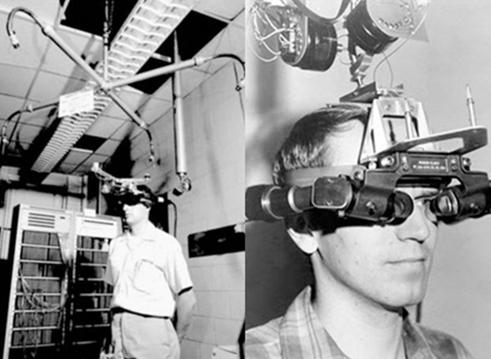
\includegraphics[width=0.5\textwidth]{figs/Sword-of-Damocles.png}
    \caption{Primer sistema RA: "Sword of Damocles" (1968)}
    \label{fig:sword_of_damocles}
\end{figure}

No obstante, el concepto formal de RA se desarrolló más tarde. En 1992, Caudell y Mizell acuñaron el término Augmented Reality en un contexto industrial, para referirse al uso de displays que asistían a operarios durante tareas complejas. Este enfoque pragmático orientó la investigación hacia sistemas útiles para tareas del mundo real, diferenciándose de la realidad virtual (RV), que propone la inmersión total en entornos digitales.

\subsection{Definición formal y primeros prototipos (1990–2000)}
Ronald Azuma estableció en 1997 la definición académica más citada de RA, basada en tres criterios fundamentales: (1) combinación de elementos reales y virtuales, (2) interacción en tiempo real y (3) registro espacial tridimensional preciso~\cite{azuma1997}. En paralelo, Paul Milgram y Fumio Kishino introdujeron el Continuo Realidad-Virtualidad, que posiciona la RA entre el entorno físico puro y la RV completa, permitiendo caracterizar distintos grados de mezcla entre ambos mundos~\cite{billinghurst2015}.

\begin{figure}[H]
    \centering
    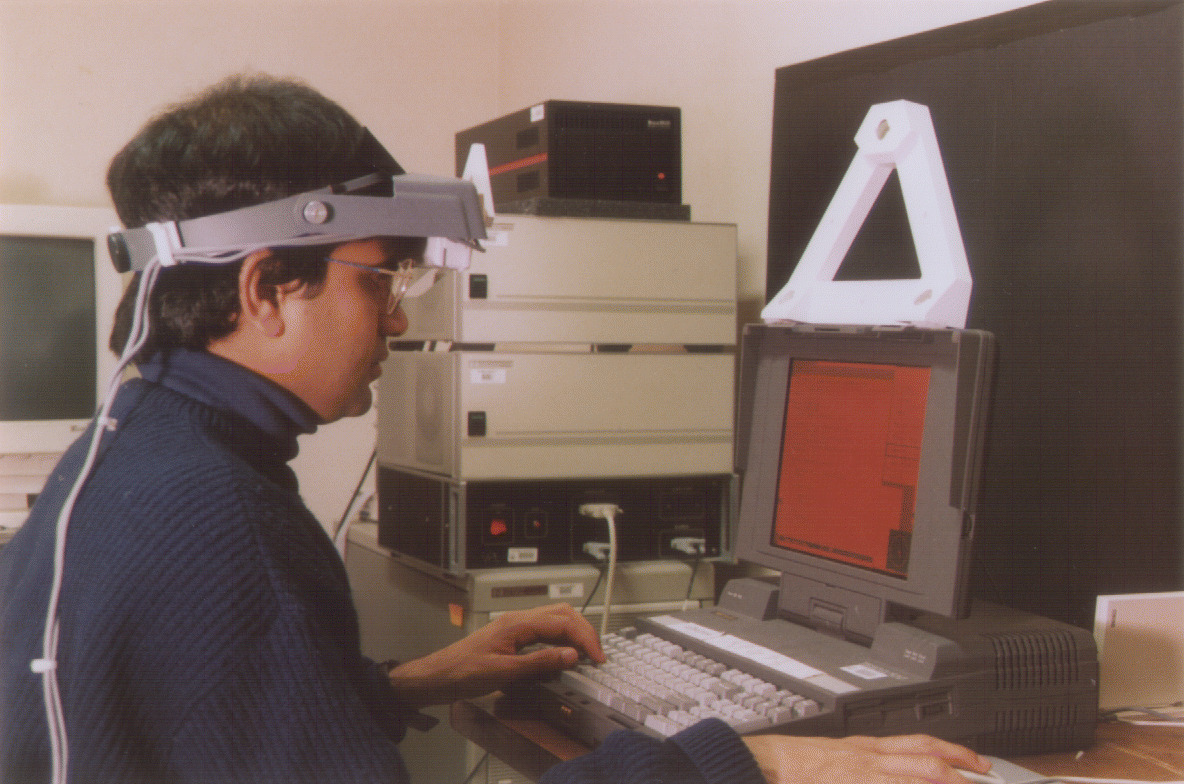
\includegraphics[width=0.6\textwidth]{figs/karma.jpg}
    \caption{Sistema KARMA para asistencia con RA (1993)}
    \label{fig:karma}
    % Fuente: Feiner et al., 1993
\end{figure}

Durante esta década se desarrollaron los primeros sistemas funcionales de RA. En 1993, el sistema KARMA, creado por Steve Feiner y su equipo, permitía la superposición de información contextual durante tareas físicas~\cite{feiner1993}. En 1997, se presentó el prototipo MARS, un sistema de RA móvil diseñado para guiar a turistas mediante visualización aumentada en tiempo real. Estas iniciativas fueron posibles gracias al desarrollo de dispositivos portables y técnicas de tracking visual.

\subsection*{Herramientas abiertas y salto a lo portátil (1999–2010)}
Uno de los hitos más relevantes en esta etapa fue el desarrollo de ARToolKit por Hirokazu Kato y Mark Billinghurst en 1999. Esta librería de código abierto permitió detectar marcadores visuales en video y superponer contenido digital 3D en tiempo real~\cite{kato1999}. Supuso una democratización de la RA, facilitando la experimentación por parte de investigadores y desarrolladores independientes.

\begin{figure}[H]
    \centering
    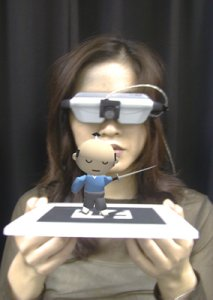
\includegraphics[width=0.3\textwidth]{figs/artoolkit.jpg}
    \caption{ARToolKit y marcadores visuales (1999)}
    \label{fig:artoolkit}
    % Fuente: Página del proyecto o artículo original
\end{figure}

Entre 2001 y 2004, surgieron los primeros sistemas de RA sobre dispositivos móviles, como PDAs y teléfonos inteligentes de primera generación. En 2003, Wagner y Schmalstieg presentaron un sistema de RA completamente autónomo en un dispositivo de mano~\cite{wagner2003}. Otros experimentos destacados fueron ARQuake (2000), un videojuego de RA en primera persona, y Invisible Train (2004), una aplicación colaborativa con varios usuarios simultáneos.


\section{La visibilización de las mujeres en el espacio urbano: una cuestión de justicia histórica}

La representación de las mujeres en el espacio urbano continúa siendo escasa. Según el proyecto europeo “Women’s Legacy”~\cite{womenslegacy2022}, impulsado desde la Conselleria d’Educació, Cultura i Esport de la Generalitat Valenciana, solo un 10\% de las calles con nombres de personas en muchas ciudades españolas están dedicadas a mujeres, y este patrón se repite en monumentos, placas conmemorativas y espacios simbólicos. 

A pesar de esta disparidad, en los últimos años han surgido iniciativas locales e institucionales orientadas a revertir esta situación. En Valencia, destaca el proyecto “Dones de Ciència”~\cite{lasnaves2020}, una colaboración entre la Universitat Politècnica de València (UPV) y Las Naves, que ha creado más de 30 murales urbanos en centros educativos para homenajear a mujeres científicas de todo el mundo. Esta intervención artística no solo embellece el entorno, sino que actúa como una herramienta pedagógica para inspirar a las nuevas generaciones. Asimismo, el Ayuntamiento de València ha promovido campañas de renombramiento de calles con nombres femeninos y la inclusión de mujeres en los itinerarios culturales y turísticos de la ciudad~\cite{ayuntamientovalencia2023}.

Por otra parte, diversas asociaciones vecinales y colectivos feministas han impulsado rutas autogestionadas por la ciudad que visibilizan las huellas femeninas en el espacio urbano. Entre ellas destaca la "Ruta Violeta de Mujeres en Valencia", organizada por la Asociación Por Ti Mujer, que recorre espacios emblemáticos ligados a la historia de las mujeres en la ciudad, promoviendo un reconocimiento público de sus contribuciones sociales y culturales~\cite{portimujer2023}.

Asimismo, la Assemblea Feminista de València ha organizado la "Ruta pels espais del Patronato de Protección a la Mujer", que recorre espacios vinculados a esta institución franquista, la cual operó durante gran parte del siglo XX bajo la tutela de la Iglesia y el Estado. Su función no era tanto proteger a mujeres víctimas de violencia como controlar y castigar a aquellas que transgredían los roles tradicionales de género. Esta ruta permite evidenciar cómo las estructuras institucionales legitimaron la exclusión, la represión y la estigmatización de mujeres consideradas "desviadas" por la moral conservadora, visibilizando así dinámicas de resistencia y memoria colectiva en la ciudad ~\cite{assemblea2023}.

Además, la "Ruta de Memorias Lesbianas", también organizada por la Assemblea Feminista de València, recorre lugares significativos para la comunidad lésbica, con el objetivo de visibilizar los derechos y experiencias de las mujeres lesbianas en la Valencia de los años 70, 80 y 90, destacando la importancia de reconocer y valorar estas luchas en la construcción de la historia urbana~\cite{assemblea2024}.

Estas rutas permiten redescubrir barrios desde una óptica feminista, incorporando historias personales, luchas sociales y legados invisibilizados. En este sentido, la plataforma DONA’m MÓN podría ser un recurso útil a implementar durante estas rutas, integrando información geolocalizada, recursos multimedia y facilitando la participación activa de las personas en la construcción de esta memoria feminista urbana. 


\subsection{Referentes femeninos en la ciudad: biografías y puntos de interés}

La aplicación propuesta busca poner en valor la figura de mujeres que, desde distintos campos del saber y la acción, han contribuido de manera decisiva al progreso de los derechos, el pensamiento y la cultura. Aunque muchas de ellas han nacido o trabajado en Valencia, su legado trasciende el ámbito local y constituye una aportación fundamental a la historia del feminismo y la igualdad. A través de la geolocalización de lugares clave asociados a sus vidas y obras, se propone una experiencia que va más allá de la información enciclopédica, para convertirse en un ejercicio de reconocimiento social y emocional de su presencia en la ciudad.

Una de las figuras destacadas es Concepción Aleixandre Ballester (1862–1952), una de las primeras mujeres médicas en España y pionera en el ámbito de la ginecología. Su activismo feminista se centró en la defensa del acceso de las mujeres a la educación y al ejercicio profesional de la medicina, algo profundamente innovador en su tiempo. Estudió en la Universidad de Valencia, donde enfrentó obstáculos institucionales por su condición de mujer, y desarrolló una intensa carrera médica y científica. El edificio histórico de la Facultad de Medicina de la Universitat de València es un lugar simbólico para recordar su figura y su lucha por la igualdad en el ámbito sanitario~\cite{guijarro2021}.

Otra mujer fundamental en la historia reciente de Valencia es Carmen Alborch (1947–2018). Fue ministra de Cultura, escritora, catedrática de Derecho Mercantil y una de las voces más influyentes del feminismo institucional en España. Su obra literaria, como \textit{Solas} (1999), promovió un feminismo humanista accesible y empático. En Valencia, dejó una impronta profunda como directora del Instituto Valenciano de Arte Moderno (IVAM), donde impulsó una política cultural abierta, plural y comprometida con la igualdad. El IVAM, por tanto, no solo representa su labor como gestora cultural, sino también su apuesta por un feminismo integrador desde las instituciones~\cite{alborch1999}.

En el ámbito de los derechos civiles, Clara Campoamor (1888–1972) ocupa un lugar esencial por su incansable lucha por el sufragio femenino, que logró defender con éxito en las Cortes Constituyentes de 1931. Si bien no tuvo una vinculación directa con Valencia, su legado ideológico inspiró a generaciones de mujeres en toda España, incluida la Comunidad Valenciana. La existencia de centros educativos como el CEIP Clara Campoamor subraya la importancia de su figura como referente pedagógico y su impacto en la formación de una conciencia feminista desde edades tempranas~\cite{gonzalez2006}.

Retrocediendo a la Edad Media, encontramos a Isabel de Villena (1430–1490), abadesa del Real Monasterio de la Trinidad y considerada la primera escritora en lengua valenciana. Su obra \textit{Vita Christi} constituye una relectura humanista del relato evangélico desde una perspectiva femenina, resaltando la figura de la Virgen y otras mujeres bíblicas. Isabel de Villena transformó el espacio monástico en un lugar de producción intelectual y espiritual liderado por mujeres, algo excepcional en su época. El Monasterio de la Trinidad, donde vivió y escribió, es un lugar clave para reivindicar la aportación femenina a la literatura y la espiritualidad valencianas~\cite{rueda2013}.

En la medicina, Manuela Solís Clarás (1888–1936) destaca por ser una de las primeras mujeres médicas de la ciudad. Ejerció en el Hospital Provincial de Valencia y fue una firme defensora del acceso de las mujeres a la formación sanitaria. Además de su práctica médica, se implicó en la divulgación científica y en la promoción de redes de apoyo entre profesionales sanitarias, en un momento en que la medicina era un espacio profundamente masculinizado~\cite{martinez2019}. El Hospital Provincial es, por tanto, un espacio idóneo para recordar su legado.

La aplicación también incluye representaciones artísticas contemporáneas de mujeres de gran relevancia internacional. Por ejemplo, Mae Jemison, primera mujer afroamericana en viajar al espacio, es homenajeada con un mural en el CEIP Torrefiel. Su figura simboliza la superación de barreras raciales y de género en los campos de la ciencia y la exploración espacial. Del mismo modo, Vandana Shiva, ecofeminista india y activista medioambiental, cuenta con un mural en el CEIP Ballester Fandos. Su lucha por la justicia ambiental, la soberanía alimentaria y los derechos de las mujeres rurales conecta con un feminismo global que también debe tener presencia en las narrativas educativas locales~\cite{shiva2005}.

“DONA’m MÓN” busca ser un vehículo para visibilizar la presencia de estas figuras en el espacio urbano, contribuyendo así a una representación más justa y equitativa de la historia y promoviendo un futuro en el que la diversidad y la igualdad sean valores fundamentales.

\begin{figure}[H]
    \centering
    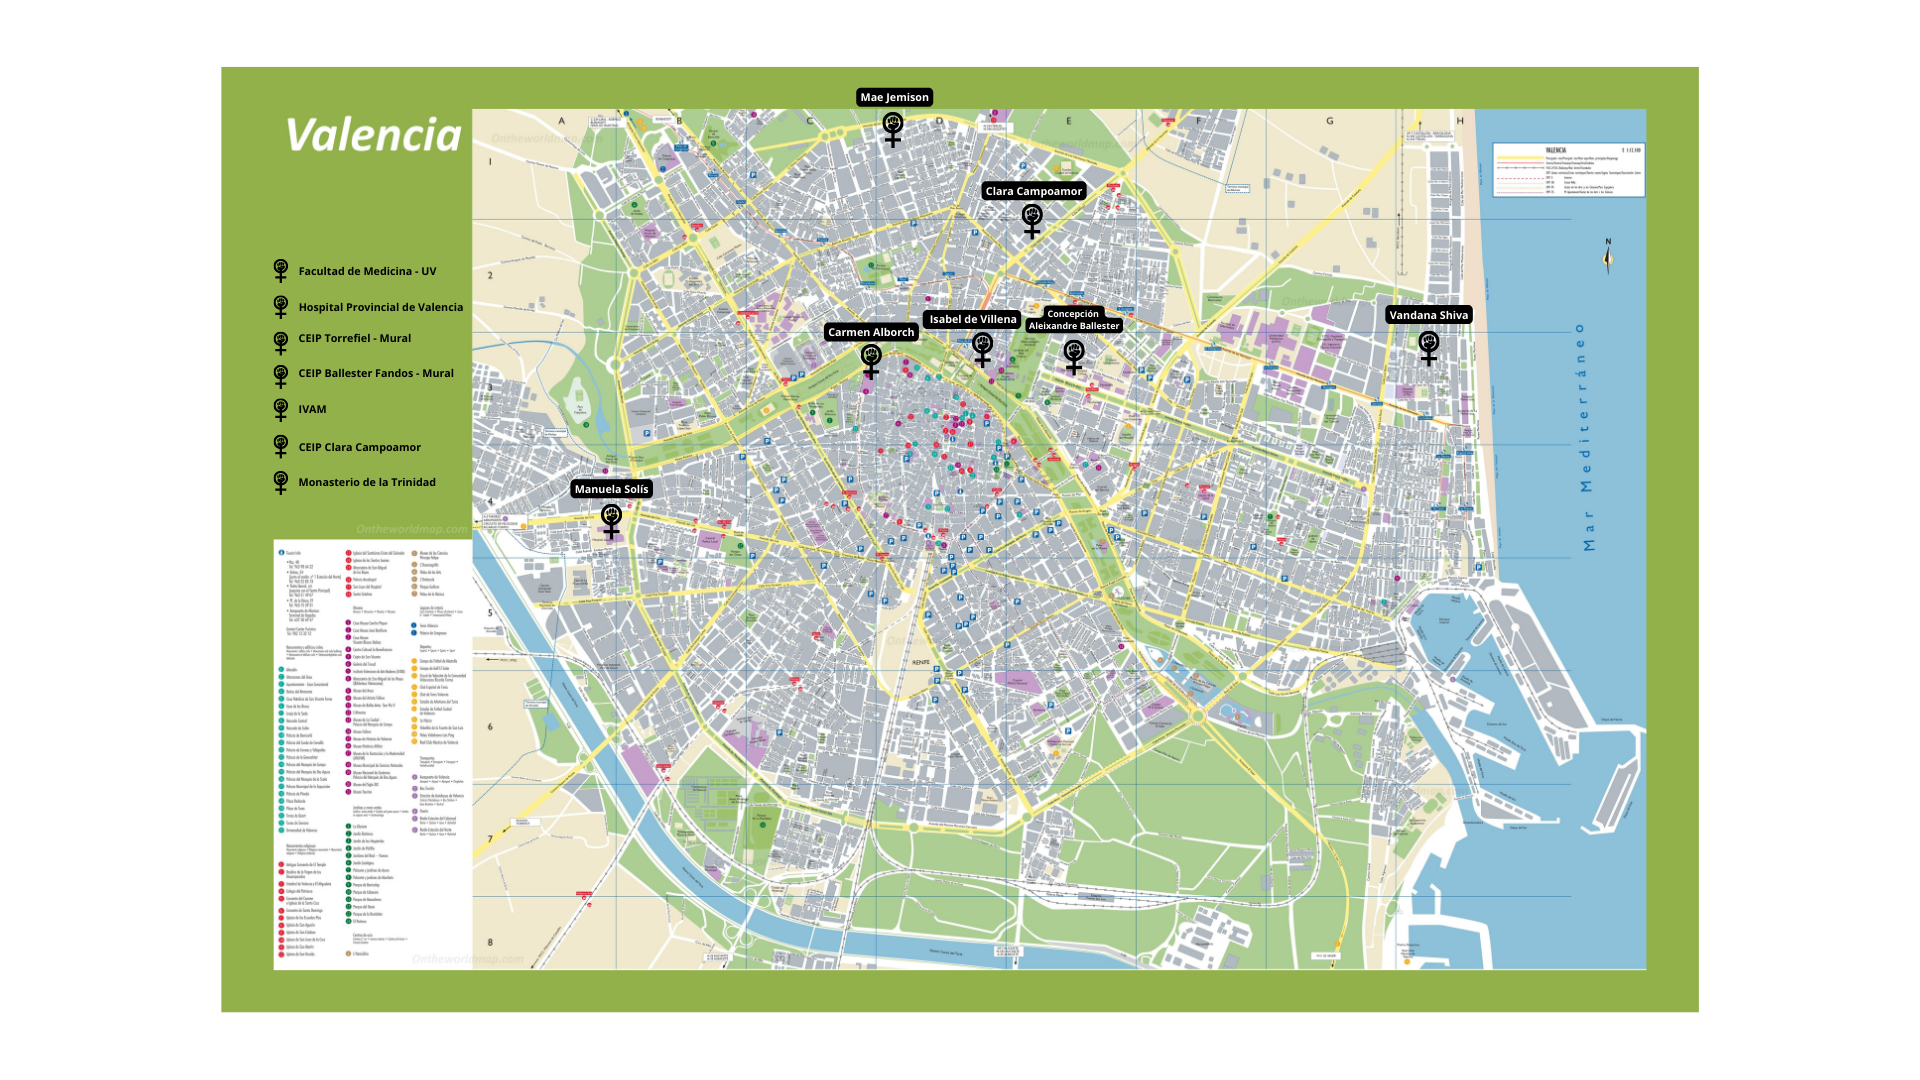
\includegraphics[width=\textwidth]{figs/mapa.png}
    \caption{Mapa de Valencia con los puntos geolocalizados de las mujeres referentes incluidos en la aplicación.}
    \label{fig:mapa_valencia_mujeres}
\end{figure}



\section{Análisis de aplicaciones similares}
% Qué aplicaciones similares hay y en qué se diferencia de ellas la propuesta

En el desarrollo de “DONA’m MÓN”, resulta esencial analizar aplicaciones existentes que, de manera similar, combinan geolocalización y realidad aumentada (RA) para ofrecer experiencias inmersivas y educativas. Este análisis nos permite identificar características, estrategias y tecnologías clave que podrían ser adaptadas para cumplir con los objetivos específicos del proyecto. A continuación, se presentan algunas aplicaciones relevantes cuyos enfoques, funcionalidades y tecnologías han inspirado aspectos concretos del diseño conceptual de este TFG.

\subsubsection{Pokémon GO}

Una de las referencias más notables es Pokémon GO, que revolucionó el mercado de aplicaciones móviles al combinar geolocalización y RA para motivar a los usuarios a explorar el mundo real. En este caso, los jugadores buscan y capturan criaturas virtuales que aparecen en puntos geográficos específicos. La aplicación también implementa un sistema de recompensas y niveles que fomenta la participación constante. Aunque el enfoque principal de Pokémon GO es el entretenimiento, su éxito demuestra cómo las tecnologías inmersivas pueden transformar la forma en que las personas interactúan con su entorno. En “DONA’m MÓN”, se busca adaptar esta dinámica de exploración y descubrimiento, pero con un enfoque educativo y cultural, utilizando los puntos de interés como portales hacia las historias de mujeres que dejaron una huella significativa en Valencia.

\begin{figure}[H]
    \centering
    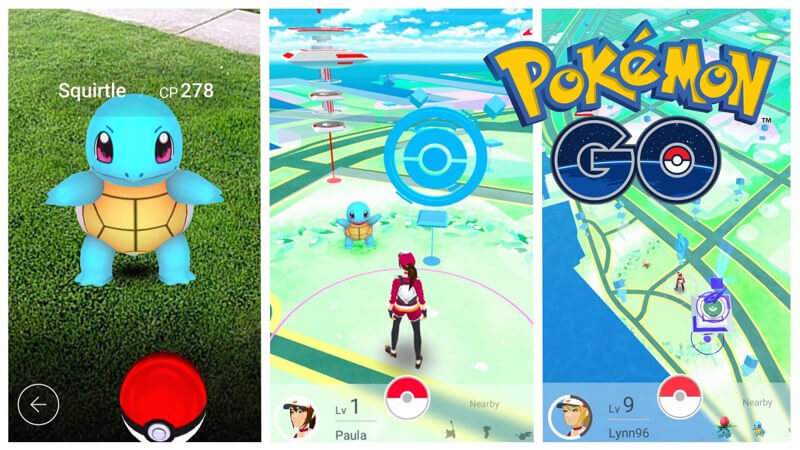
\includegraphics[width=0.5\textwidth]{figs/pokemon_go.jpg}
    \caption{Interfaz de Pokémon GO mostrando un entorno real aumentado con la aparición de un Pokémon virtual y también el entorno virtual del juego.}
    \label{fig:pokemon_go}
\end{figure}

\subsubsection{Streetmuseum}

Por otro lado, Streetmuseum es una aplicación que también aprovecha la RA, pero con un objetivo más centrado en la historia y la cultura. Esta herramienta permite a los usuarios visualizar imágenes y escenas históricas superpuestas al paisaje actual, ofreciendo una perspectiva del pasado en tiempo real. La capacidad de conectar visualmente el entorno moderno con eventos y figuras históricas es una inspiración directa para el proyecto. En nuestro proyecto, esta idea se adapta al permitir que los usuarios accedan a contenido multimedia –como imágenes, textos y modelos 3D– que contextualice la vida y obra de las mujeres en cada ubicación geolocalizada.

\begin{figure}[H]
    \centering
    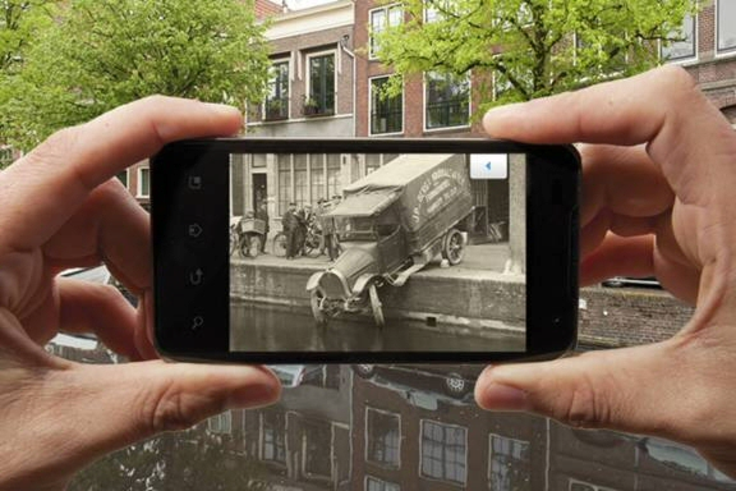
\includegraphics[width=0.5\textwidth]{figs/streetmuseum.png}
    \caption{Ejemplo de Streetmuseum: visualización de una escena histórica superpuesta sobre el entorno actual de la ciudad.}
    \label{fig:streetmuseum}
\end{figure}

\subsubsection{CultuAR}

CultuAR, desarrollada por la empresa española AR Vision, es una aplicación que combina la geolocalización con la realidad aumentada para ofrecer visitas culturales interactivas en más de 200 municipios. Mediante la cámara del dispositivo, los usuarios pueden visualizar reconstrucciones históricas, personajes del pasado o información multimedia superpuesta al entorno real. Una de sus características más valiosas es la capacidad de personalizar rutas culturales por municipios, integrando elementos inmersivos que enriquecen la experiencia turística y patrimonial. Esta aplicación destaca por su integración fluida con el entorno urbano y su enfoque didáctico, lo que representa una clara inspiración para DONA'm MÓN en cuanto a accesibilidad y diseño de experiencias geolocalizadas con RA.

\begin{figure}[H]
    \centering
    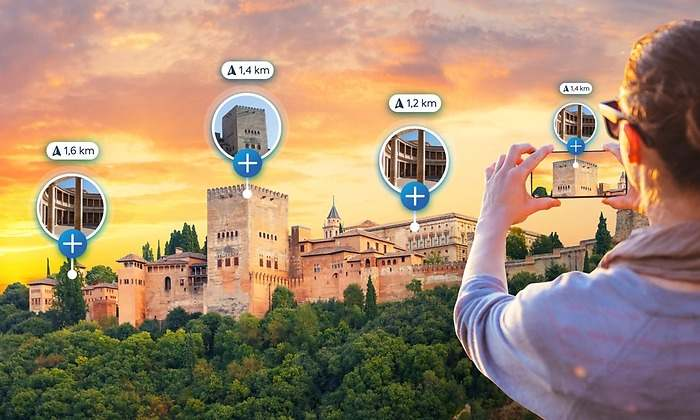
\includegraphics[width=0.5\textwidth]{figs/cultuar.jpeg}
    \caption{Captura de CultuAR mostrando información sobre un monumento en el entorno real.}
    \label{fig:cultuar}
\end{figure}

\subsubsection{Historypin}

Finalmente, Historypin se presenta como una plataforma colaborativa que permite a los usuarios subir y explorar fotografías, eventos y recuerdos históricos asociados a ubicaciones específicas. Lo más destacable de esta aplicación es su enfoque participativo, donde los usuarios pueden contribuir activamente al contenido disponible. Este modelo de colaboración inspira la posibilidad de que, en futuras versiones de “DONA’m MÓN”, los usuarios también puedan agregar información o enriquecer las narrativas existentes sobre mujeres de Valencia, convirtiendo la aplicación en una herramienta dinámica y viva.

\begin{figure}[H]
    \centering
    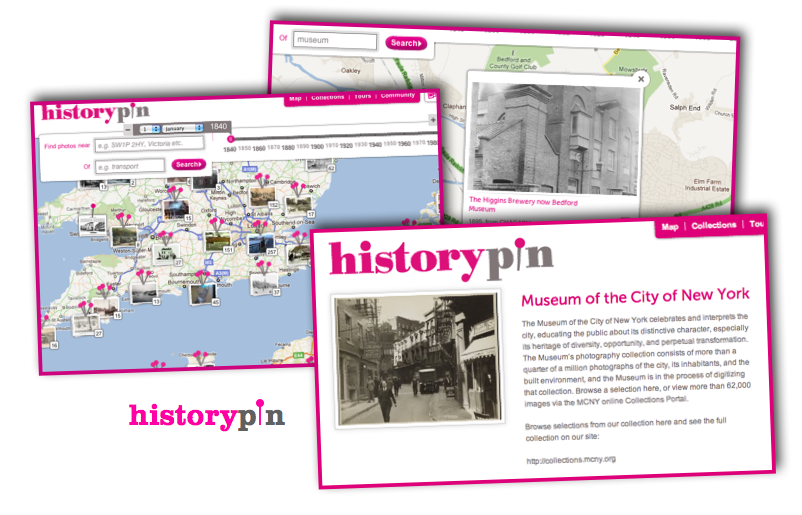
\includegraphics[width=0.5\textwidth]{figs/history-pin.png}
    \caption{Interfaz de Historypin donde se visualizan fotografías históricas asociadas a ubicaciones reales en el mapa y su detalle de contenido.}
    \label{fig:historypin}
\end{figure}
\subsubsection{}

Estas cuatro aplicaciones ilustran diversas maneras de utilizar la tecnología para crear experiencias inmersivas e interactivas. Cada una de ellas presenta fortalezas únicas que se alinean, en mayor o menor medida, con los objetivos de DONA'm MÓN. De Pokémon GO tomamos la dinámica de exploración y gamificación; de Streetmuseum, la idea de superponer contenido histórico en el entorno actual; de CultuAR, el uso efectivo de RA para la divulgación cultural local; y de Historypin, el potencial de colaboración comunitaria. Esta combinación de estrategias y conceptos pretende hacer de DONA'm MÓN una aplicación única que conecte a los usuarios con la historia de manera inclusiva, educativa e innovadora.



\section{Tecnologías}
% Análisis crítico de las tecnologías y sistemas de despliegue posibles y por qué se han seleccionado unas concretas.
En este apartado se analizan las tecnologías disponibles y las soluciones existentes en el mercado que pueden ser aplicadas al desarrollo de la aplicación móvil. Este análisis incluye una revisión de herramientas de geolocalización, realidad aumentada, bases de datos y frameworks de desarrollo multiplataforma. La selección de las tecnologías se justifica considerando la funcionalidad, compatibilidad y eficiencia necesarias para cumplir con los objetivos del proyecto.

\subsection{Plataformas de desarrollo de aplicaciones móviles}

Una de las decisiones fundamentales en cualquier proyecto de ingeniería de software es la elección de la tecnología base sobre la cual se construirá la aplicación. Esta decisión afecta directamente a la arquitectura general, la experiencia de usuario, la mantenibilidad del código y la escalabilidad futura del sistema. En el contexto de este proyecto, se evaluaron varias opciones para el desarrollo de una aplicación móvil multiplataforma que integrase geolocalización, funcionalidades de realidad aumentada, y una interfaz moderna, accesible y responsiva.

\textbf{Unity.} Unity es un motor de desarrollo multiplataforma ampliamente utilizado en los ámbitos del videojuego, simulación y experiencias interactivas en tiempo real. Su potencia radica en su motor gráfico, que permite renderizar contenido 3D de alta calidad, así como en su flexibilidad para implementar lógica de aplicación mediante scripts en C\#. Unity ofrece soporte directo para tecnologías de realidad aumentada a través de módulos como AR Foundation, que actúan como capa de abstracción sobre ARKit (iOS) y ARCore (Android), permitiendo así desarrollar una única base de código RA para múltiples plataformas.

En lo relativo a interfaces de usuario, Unity ha evolucionado en los últimos años. Su sistema tradicional basado en el Canvas permitía crear interfaces gráficas bidimensionales, pero con limitaciones de estilo y escalabilidad. Como respuesta a estas deficiencias, se introdujo UI Toolkit, un nuevo sistema de interfaz basado en un modelo declarativo, inspirado en tecnologías web como HTML y CSS. UI Toolkit permite separar la lógica de presentación del comportamiento, definiendo componentes visuales reutilizables y estilos en archivos dedicados. A pesar de estas mejoras, el desarrollo de interfaces ricas, formularios interactivos y navegación compleja continúa siendo menos eficiente que en frameworks específicos para aplicaciones móviles.

\textbf{React Native.} React Native es un framework desarrollado por Meta (anteriormente Facebook) para el desarrollo de aplicaciones móviles multiplataforma utilizando JavaScript y el modelo de componentes de React. Permite crear interfaces de usuario nativas reutilizando componentes declarativos que se renderizan mediante puentes hacia los componentes nativos de Android e iOS. Una de las grandes ventajas de React Native es su arquitectura reactiva, que permite gestionar estados complejos de forma eficiente, manteniendo la UI sincronizada con los datos de la aplicación.

En combinación con Expo, un conjunto de herramientas que facilita la creación y prueba de aplicaciones React Native, es posible desarrollar aplicaciones sin necesidad de compilar ni configurar código nativo. Esto permite utilizar herramientas como Expo Go para probar la aplicación directamente en un dispositivo físico mediante código QR, lo que acelera significativamente el flujo de desarrollo. React Native es especialmente potente para construir interfaces modernas, personalizadas y adaptables, con soporte para navegación compleja, formularios, animaciones y estilos dinámicos.

\textbf{Flutter.} Flutter es un framework desarrollado por Google para construir aplicaciones multiplataforma desde una única base de código. Utiliza el lenguaje Dart, y su arquitectura se basa en un sistema de renderizado propio que dibuja todos los elementos de la UI desde cero, lo que garantiza uniformidad visual entre plataformas. Flutter ofrece una amplia colección de widgets personalizables y anima la creación de interfaces complejas de forma declarativa y eficiente.

Aunque Flutter no fue la opción elegida para este proyecto, se considera una alternativa competitiva frente a React Native. Sin embargo, su adopción requiere dominar el lenguaje Dart, y su integración con tecnologías de realidad aumentada aún está en evolución en comparación con la madurez del ecosistema de Unity o la compatibilidad simplificada que ofrece React Native con herramientas web como AR.js y A-Frame.

\textbf{Desarrollo de interfaz de usuario y elección final.} Una parte crucial del proyecto es la interfaz gráfica de usuario, dado que la aplicación está destinada a un público general y debe facilitar la navegación intuitiva, la visualización de datos geográficos y el acceso a contenidos de realidad aumentada. Si bien Unity, especialmente con UI Toolkit, ofrece un entorno funcional para construir interfaces gráficas, su enfoque está más orientado a interacciones en entornos tridimensionales y menos a la gestión de flujos de navegación o formularios comunes en aplicaciones móviles.

Por el contrario, React Native destaca precisamente en este tipo de interfaz. Su modelo declarativo, su sistema de componentes reutilizables, su integración con herramientas modernas de desarrollo (como React Navigation, Redux o Context API), y su compatibilidad con Expo, permiten construir aplicaciones móviles escalables y con una experiencia de usuario optimizada.

Por estos motivos, y tras un análisis técnico detallado, se decidió utilizar React Native con Expo como entorno principal de desarrollo para esta aplicación, reservando el uso de tecnologías gráficas (como la realidad aumentada) a componentes embebidos que se integran dentro de esta arquitectura general. Esta elección permite combinar la robustez de React para la UI con la flexibilidad de integrar experiencias multimedia mediante tecnologías web.

\subsection{Geolocalización}

La geolocalización es uno de los pilares fundamentales de la aplicación, ya que permite situar puntos de interés específicos en un mapa, facilitando que los usuarios exploren la ciudad de Valencia mientras descubren la historia de mujeres destacadas. Para implementar esta funcionalidad, existen diversas herramientas ampliamente utilizadas en el desarrollo de aplicaciones móviles:

\begin{itemize}
    \item \textbf{Google Maps API}: Es una solución robusta y versátil que permite integrar mapas interactivos, obtener datos de ubicación en tiempo real y personalizar la visualización según las necesidades del proyecto. Ofrece documentación detallada y soporte técnico, lo que facilita su integración. Sin embargo, su principal desventaja es que su plan gratuito únicamente se ofrece durante un periodo de prueba de corta duración y su coste se incrementa en proyectos con un gran volumen de usuarios o solicitudes~\cite{googlemaps2024}.
    \item \textbf{Mapbox}: Alternativa potente que combina funcionalidades avanzadas, un alto nivel de personalización estética y una política de precios más flexible que Google Maps API, ya que su plan gratuito no tiene un límite de tiempo. Es especialmente útil en aplicaciones que requieren un diseño visual distintivo. No obstante, su integración puede resultar más compleja para desarrolladores con poca experiencia~\cite{mapbox2024}.
    \item \textbf{OpenStreetMap (OSM)}: Opción de código abierto que permite el acceso y uso gratuito de datos cartográficos, además de ofrecer un alto nivel de personalización. Esta plataforma colaborativa es especialmente adecuada para proyectos con presupuestos limitados o académicos, ya que no implica costes de licencia. Aunque carece de algunas funcionalidades avanzadas nativas, como el enrutamiento en tiempo real o servicios de geolocalización enriquecidos, su flexibilidad y libertad de uso la convierten en una solución funcional y accesible~\cite{osm2024}.
    \item \textbf{Mapas nativos del dispositivo con React Native}: Esta opción permite aprovechar las capacidades de geolocalización del propio sistema operativo del dispositivo móvil (iOS o Android) mediante bibliotecas como react-native-maps. Es una solución eficiente y ligera, que facilita la integración con el hardware del dispositivo y proporciona una experiencia fluida. Además, evita costes derivados de servicios externos, lo que la convierte en una alternativa atractiva para proyectos con recursos limitados~\cite{reactnativemaps2024}.
\end{itemize}

En este proyecto se ha optado por utilizar mapas nativos con React Native, ya que permiten una integración directa con la aplicación móvil, ofrecen un rendimiento óptimo, y eliminan la dependencia de servicios externos de pago. Esta elección responde a criterios de eficiencia, sostenibilidad económica y control sobre el desarrollo.

\subsection{Realidad Aumentada (RA)}

Una vez definida la arquitectura general de la aplicación y confirmado el uso de React Native como entorno principal de desarrollo, fue necesario analizar detalladamente qué tecnologías de realidad aumentada (RA) podían integrarse de forma eficiente, respetando las limitaciones del ecosistema de desarrollo adoptado. Uno de los objetivos fundamentales era conservar la compatibilidad con Expo Go, evitando procesos de compilación nativa que dificultasen el flujo de desarrollo iterativo. Bajo esta premisa, se realizó un estudio de las distintas alternativas existentes, evaluando tanto su madurez técnica como su grado de integración con React Native.

\textbf{Realidad aumentada con tecnologías nativas.}
Las soluciones nativas ofrecen, en general, el mayor grado de precisión, rendimiento y acceso a capacidades avanzadas del dispositivo. Entre estas destacan ARKit (para dispositivos iOS) y ARCore (para Android), los kits de desarrollo oficial proporcionados por Apple y Google, respectivamente. Ambas plataformas permiten el seguimiento del entorno, la detección de planos horizontales y verticales, la oclusión de objetos virtuales con respecto al entorno físico, el anclaje espacial y la iluminación adaptativa. Estas herramientas están diseñadas para crear experiencias inmersivas de alta calidad y son ampliamente utilizadas en entornos profesionales y comerciales.

Sin embargo, una de sus limitaciones fundamentales es su naturaleza monoplataforma. Para desarrollar una aplicación de RA que funcione tanto en Android como en iOS, sería necesario implementar dos versiones independientes, o bien utilizar un entorno unificador como Unity, que permite compilar una única base de código para múltiples sistemas operativos.

Unity, a través de su módulo AR Foundation, permite abstraer las diferencias entre ARKit y ARCore, y desarrollar experiencias RA multiplataforma con una arquitectura común. Unity es particularmente potente en términos de renderizado gráfico, gestión de modelos tridimensionales, simulación física y animación en tiempo real, por lo que constituye una de las herramientas más robustas para el desarrollo de RA avanzada.

No obstante, su integración con aplicaciones desarrolladas en React Native es compleja. El enfoque convencional implicaría desarrollar toda la aplicación en Unity, lo cual, como se ha discutido anteriormente, penaliza la usabilidad y escalabilidad de la interfaz. Por este motivo, se exploró también la posibilidad de utilizar Unity como una librería nativa embebida dentro de una aplicación React Native.

\textbf{Unity como librería nativa integrada en React Native.}
Unity permite exportar un proyecto como una librería nativa —un archivo .aar para Android o .framework para iOS— que puede integrarse dentro de una aplicación móvil desarrollada con otras tecnologías, como React Native. Este enfoque, conocido como Unity as a Library, ofrece la posibilidad de desarrollar únicamente la parte de RA en Unity y exponerla como un módulo invocable desde la aplicación principal.

Mediante este patrón arquitectónico, es posible mantener la lógica general y la interfaz de usuario desarrolladas en React Native, y delegar en Unity únicamente el renderizado y gestión de la escena RA. La comunicación entre ambos entornos se realiza mediante puentes nativos que deben implementarse en Java/Kotlin (para Android) y Objective-C/Swift (para iOS).

Este enfoque ha sido demostrado en proyectos como react-native-unity, que ofrecen ejemplos funcionales de integración, así como en la documentación oficial de Unity (Unity as a Library). No obstante, esta integración presenta múltiples desafíos técnicos:

\begin{itemize}
    \item Es necesario ejectar el proyecto Expo, abandonando así la posibilidad de utilizar Expo Go y el flujo de desarrollo simplificado que ofrece.
    \item La configuración del proyecto requiere conocimientos avanzados en desarrollo nativo para cada plataforma.
    \item La integración y sincronización de eventos entre Unity y React Native debe implementarse manualmente.
\end{itemize}

Por tanto, aunque Unity como librería nativa representa una solución muy potente desde el punto de vista gráfico y funcional, su coste de integración y mantenimiento dentro de una arquitectura basada en React Native la convierte en una opción poco viable para este proyecto, cuyo foco está en la accesibilidad, rapidez de desarrollo y compatibilidad multiplataforma sin compilación nativa.

\textbf{Realidad aumentada en React Native con tecnologías web.}
En busca de una alternativa más ligera y plenamente compatible con React Native y Expo, se optó por explorar las soluciones basadas en tecnologías web. Una de las más destacadas es AR.js, una librería de código abierto que permite implementar experiencias de RA directamente en navegadores móviles, sin necesidad de acceso a capas nativas. AR.js se basa en WebGL, Three.js y A-Frame, y permite implementar RA sobre marcadores visuales (marker-based AR) mediante la detección de patrones gráficos como Hiro, Kanji o diseños personalizados.

Complementando AR.js, el framework A-Frame facilita la construcción declarativa de escenas 3D y RA mediante HTML. Permite importar modelos .glb, añadir iluminación, cámaras, interacciones y animaciones sin necesidad de escribir código complejo de bajo nivel. Esta aproximación reduce significativamente la barrera de entrada al desarrollo de RA, y se adapta perfectamente al modelo de desarrollo web moderno.

Las escenas construidas con A-Frame y AR.js pueden ser desplegadas como aplicaciones web estáticas (por ejemplo, en GitHub Pages), e integradas dentro de la aplicación React Native utilizando el componente WebView, que actúa como un navegador embebido. Este enfoque permite mantener la lógica general y la interfaz de la aplicación dentro del ecosistema de React Native, mientras que la experiencia de RA se encapsula como una unidad independiente, reutilizable y fácilmente actualizable.

\textbf{Viro React.}
Otra alternativa evaluada fue Viro React, un framework orientado a la creación de experiencias inmersivas en RA y realidad virtual directamente en React Native. Viro permite cargar modelos 3D, definir cámaras, aplicar animaciones, detectar superficies, y renderizar objetos virtuales en función del entorno físico. Su enfoque declarativo está alineado con la filosofía de React y ofrece un entorno de desarrollo intuitivo para experiencias visuales.

No obstante, Viro no es compatible con Expo Go, ya que depende de módulos nativos que requieren compilar la aplicación. Para utilizarlo, es necesario ejectar el proyecto y utilizar herramientas como EAS Build para generar versiones personalizadas de la app. Esta necesidad de compilación rompe el flujo de desarrollo ágil basado en Expo y contradice uno de los principios técnicos fundamentales del proyecto: evitar configuraciones nativas complejas para preservar la portabilidad y escalabilidad del sistema.

\textbf{Elección final.}
Después de un análisis riguroso, se optó por utilizar AR.js combinado con A-Frame, integrados en la aplicación React Native mediante un componente WebView. Esta solución permite cumplir los objetivos funcionales de la aplicación (visualización de modelos 3D sobre marcadores físicos), respetando al mismo tiempo los requisitos técnicos del entorno (compatibilidad con Expo, desarrollo ágil, y arquitectura limpia).

La elección de esta tecnología responde a criterios técnicos sólidos:

\begin{itemize}
    \item Portabilidad total: la experiencia RA se ejecuta en el navegador y es accesible desde cualquier dispositivo moderno.
    \item Desacoplamiento arquitectónico: la escena RA es independiente del código base de la aplicación.
    \item Facilidad de mantenimiento: se pueden actualizar las escenas de RA sin necesidad de recompilar la app.
    \item Compatibilidad con Expo Go: se preserva el flujo de desarrollo iterativo y multiplataforma.
\end{itemize}

En resumen, esta arquitectura permite combinar las ventajas del desarrollo móvil moderno (mediante React Native) con la flexibilidad de tecnologías web para RA, consiguiendo una solución técnica equilibrada, funcionalmente completa y sostenible a largo plazo.

\subsection{Base de Datos}

\subsection{Arquitectura de persistencia y gestión de datos}

En el desarrollo de esta aplicación se ha optado por una arquitectura desacoplada que separa claramente el frontend y el backend. El frontend se implementa en React Native, lo que permite el despliegue multiplataforma en dispositivos móviles, mientras que el backend se desarrolla en Django, un framework web de alto nivel que facilita la creación de aplicaciones robustas y seguras~\cite{django2024}.

\subsubsection{Persistencia de datos en entornos relacionales y no relacionales}

La persistencia de datos es un aspecto fundamental en el desarrollo de aplicaciones que requieren almacenar información de manera duradera. Existen dos enfoques principales para gestionar esta persistencia: las bases de datos relacionales, que estructuran la información en tablas con relaciones definidas mediante claves, y las bases de datos no relacionales, que permiten una mayor flexibilidad al almacenar los datos en formatos como documentos, grafos o pares clave-valor~\cite{elmasri2017}. 

Las bases de datos relacionales son especialmente adecuadas cuando los datos presentan una estructura definida, relaciones entre entidades y necesidad de integridad referencial, mientras que las no relacionales ofrecen ventajas en contextos donde la escalabilidad horizontal, la alta disponibilidad o la variabilidad en los esquemas de datos son prioritarias~\cite{stonebraker2011}.

\subsubsection{Django y la arquitectura MVT}

Django se basa en la arquitectura Modelo–Vista–Plantilla (MVT), un patrón similar al clásico MVC (Model–View–Controller), adaptado al ecosistema web de Python~\cite{vincent2020}. Este patrón organiza el código en tres componentes:

\begin{itemize}
    \item \textbf{Modelo (Model):} Define la estructura de los datos y su comportamiento a través de clases Python, que se traducen automáticamente en tablas mediante el ORM (Object-Relational Mapping) de Django.
    \item \textbf{Vista (View):} Gestiona la lógica de negocio y responde a las solicitudes HTTP, procesando la información que llega desde el frontend.
    \item \textbf{Plantilla (Template):} Presenta la información al usuario utilizando HTML enriquecido con etiquetas dinámicas, aunque en este proyecto su papel es mínimo, ya que la interfaz se renderiza completamente en React Native.
\end{itemize}

La interacción entre Django y la base de datos está mediada por su ORM, lo que permite manipular los datos mediante objetos Python en lugar de consultas SQL explícitas. Esta capa de abstracción incrementa la seguridad —previniendo ataques como la inyección SQL— y facilita el mantenimiento del código~\cite{vincent2020}.

\subsubsection{Sistema de Gestión de Bases de Datos: MySQL}

Para este proyecto se ha elegido MySQL como sistema de gestión de bases de datos relacional (SGBDR), debido a su madurez, rendimiento y plena compatibilidad con Django~\cite{oracle2023}. MySQL permite estructurar los datos de manera eficiente y soporta operaciones complejas con múltiples relaciones entre tablas, lo que resulta fundamental para gestionar tanto la información relacionada con las figuras históricas como los datos de geolocalización, multimedia y analíticas del uso de la app.

La configuración entre Django y MySQL se realiza mediante el uso de controladores compatibles (como \texttt{mysqlclient}), lo que asegura una integración fluida y un rendimiento óptimo.

\subsubsection{Comparativa entre sistemas de bases de datos}

A continuación se muestra una tabla comparativa entre los principales sistemas de gestión de bases de datos considerados:

\begin{table}[H]
    \centering
    \begin{tabular}{|l|c|c|c|c|}
        \hline
        \textbf{Característica} & \textbf{SQLite} & \textbf{MySQL} & \textbf{MariaDB} & \textbf{MongoDB} \\ \hline
        Tipo & Relacional & Relacional & Relacional & No relacional \\ \hline
        Escalabilidad & Baja & Alta & Alta & Muy alta \\ \hline
        Rendimiento & Medio & Alto & Muy alto & Alto \\ \hline
        Integridad referencial & Sí & Sí & Sí & No \\ \hline
        Compatibilidad Django & Nativa & Completa & Completa & Parcial (con plugins) \\ \hline
        Flexibilidad de esquema & Baja & Media & Media & Alta \\ \hline
        Facilidad de configuración & Muy fácil & Media & Media & Media \\ \hline
        Comunidad y soporte & Moderada & Muy activa & Activa & Muy activa \\ \hline
    \end{tabular}
    \caption{Comparativa entre SQLite, MySQL, MariaDB y MongoDB~\cite{elmasri2017, mariadb2023, mongodb2024}.}
    \label{tabla:comparativa_bases_datos}
\end{table}

\subsubsection{Consideraciones sobre otras tecnologías: MariaDB, SQLite, MongoDB y Cassandra}

Aunque inicialmente se contempló el uso de MariaDB, una bifurcación de MySQL con mejoras en rendimiento y licencias completamente abiertas, finalmente se optó por MySQL por razones de compatibilidad institucional y soporte técnico~\cite{mariadb2023}. SQLite, si bien está soportada nativamente por Django y resulta útil en fases de desarrollo o en aplicaciones de bajo requerimiento, no ofrece la escalabilidad ni la gestión de concurrencia necesarias para este proyecto~\cite{django_sqlite2024}. 

En cuanto a las bases de datos no relacionales, cabe mencionar tecnologías como MongoDB y Cassandra. MongoDB, basada en documentos JSON, es ampliamente utilizada en aplicaciones que requieren estructuras de datos flexibles y cambios frecuentes en el esquema~\cite{mongodb2024}. Cassandra, por su parte, está orientada a entornos distribuidos con grandes volúmenes de datos y alta disponibilidad~\cite{cassandra2023}. Sin embargo, el enfoque relacional fue considerado más adecuado para las necesidades estructuradas y normalizadas del presente trabajo.

\vspace{1em}